\documentclass{article}
\usepackage[letterpaper,margin=1in]{geometry}
\usepackage{xcolor}
\usepackage{natbib}
\usepackage{graphicx}
\setlength{\bibsep}{0.0pt}
\patchcmd{\thebibliography}
  {\settowidth}
  {\setlength{\itemsep}{-2pt plus 0.05pt}\settowidth}
  {}{}
\apptocmd{\thebibliography}
  {\small}
  {}{}


\usepackage{fancyhdr}
\usepackage{tgschola} % or any other font package you like
\usepackage{lastpage}

\pagestyle{fancy}
\fancyhf{}
\fancyhead[C]{%
  \footnotesize\sffamily
  \yourname\quad
  Web: \textcolor{blue}{\yourweb}\quad
  E-mail: \textcolor{blue}{\youremail}}

\cfoot{Page \thepage\ of \pageref{LastPage}}
%\setlength\parindent{0pt}

\newcommand{\soptitle}{Statement of Purpose}
\newcommand{\yourname}{Md Mustafizur Rahman}
\newcommand{\youremail}{\href{mailto:nahid@utexas.edu}{nahid@utexas.edu}}
\newcommand{\yourweb}{\url{https://www.ischool.utexas.edu/~nahid}}

\newcommand{\statement}[1]{\par\medskip
  \underline{\textcolor{blue}{\textbf{#1:}}}\space
}

\usepackage[
  colorlinks,
  breaklinks,
  citecolor = black,
  pdftitle={\yourname - \soptitle},
  pdfauthor={\yourname},
  urlcolor=blue,
  colorlinks=true,
  linkcolor=black,
  unicode
]{hyperref}


\begin{document}
\begin{center}\LARGE\soptitle\\
\small University Graduate Continuing Fellowship
\end{center}
\hrule
\vspace{1pt}
\hrule height 1pt
\bigskip

%\noindent{\bf Problem Statement:} With the incredible growth of information in digital media (e.g. the rise of the Web, email, Twitter, etc.), information retrieval (IR) systems (e.g. Google, Bing etc.) for searching all of this vast information have become an integral component in modern society for efficiently finding desired information. To reliably evaluate IR systems, existing methodology relies on people manually annotating the relevance of search results to queries. However, collecting a manual judgment for so many possible queries and search results is infeasible given the large size of today's information repositories. Consequently, there is an urgent need for better IR evaluation methods which are both cost-effective and highly scalable. While commercial search engines (e.g., Google) may effectively handle this problem for search problems of commercial interest (e.g., Web search), search evaluation in many other areas has been neglected (e.g., searching oral history). My doctoral research focuses on developing low-cost IR evaluation methods by integrating artificial intelligence (AI) techniques with human annotation. \\
 
\noindent{\bf Background:} With the massive growth of digital information (e.g. the rise of the Web, email, and Twitter, etc.), accurate and efficient search systems such as Google have become critical to the functioning of modern society. While today's corporate search engines already provide search solutions in many areas of commercial interest (e.g., Web search), many important search problems lie beyond commercial interest (e.g., searching oral history). The field of information retrieval (IR) research broadly investigates the science of engineering effective search systems. \\

\noindent{\bf Problem Statement:} Development of new search algorithms requires an evaluation framework in which A/B testing of new vs. existing algorithms can be reliably performed. While today's search evaluation methodology is reliable, it relies heavily upon people manually annotating the relevance of many search results, which is slow and expensive. Moreover, this practice has become increasingly infeasible as digital collections have grown ever-larger. Consequently, there is an urgent need today for better IR evaluation methods which are both cost-effective and reliable. My doctoral research focuses on developing low-cost yet reliable IR evaluation methods by integrating state-of-the-art artificial intelligence (AI) techniques with traditional human annotation. \\
 
%\noindent{\bf Background:} Traditional evaluation of IR systems (\cite{sanderson2010test}) relies on the construction of a {\em test collection}: a document collection, a set of search topics expressing a range of possible information needs of users, and human judgments of document relevance for those search topics. The long-standing practice for developing test collections is organizing a {\em shared task}, where multiple IR systems participate and each of those systems provides a ranked list of documents according to their topical relevance. To reduce the manual effort in a shared task, a conventional approach known as {\em pooling}, is applied where only a pool of the top-ranked documents, retrieved by each of the IR systems, are judged by human annotators. However, organizing a shared task is difficult, slow, and expensive. On the other hand, pooling based approaches are known to have a strong bias towards the best performing IR system, since those methods rely on the ranked list of documents provided by the participating IR systems to select documents for human judgment. \\ 
\noindent{\bf  Current Work (1 of 2):} 
My first line of research toward this goal was submitted in September 2018 to the Journal of the Association for Information Science and Technology (JASIS\&T) \cite{DBLP:journals/corr/abs-1801-05605}. In this work, I seek to reduce the human annotation effort needed to evaluate IR systems by using a sophisticated AI technique, known as {\it active learning}.  Specifically, rather than relying entirely on human annotators to judge search results, I propose an amalgam of human annotation and AI automation. {\bf Figure \ref{Figure:IR_evaluation}} illustrates the difference between the proposed hybrid model and traditional IR evaluation. This hybrid system works as follows. Firstly, during the initial stages, the system selects a set of search results for human judges to annotate which will be most informative for training the AI model. After training the AI model using these human judgments, we use the AI system to automatically judge the remaining search results. Experimental evaluation over various dataset shows that the AI system achieves 90\% accuracy in annotating search results when their human counterparts provide 60\% fewer annotations. 

%https://docs.google.com/drawings/d/1ABdqScOC_silAxZhIAiZ7ve9yJYr63_OFczxwliox34/edit?usp=sharing
\begin{figure*}[ht]
\centerline{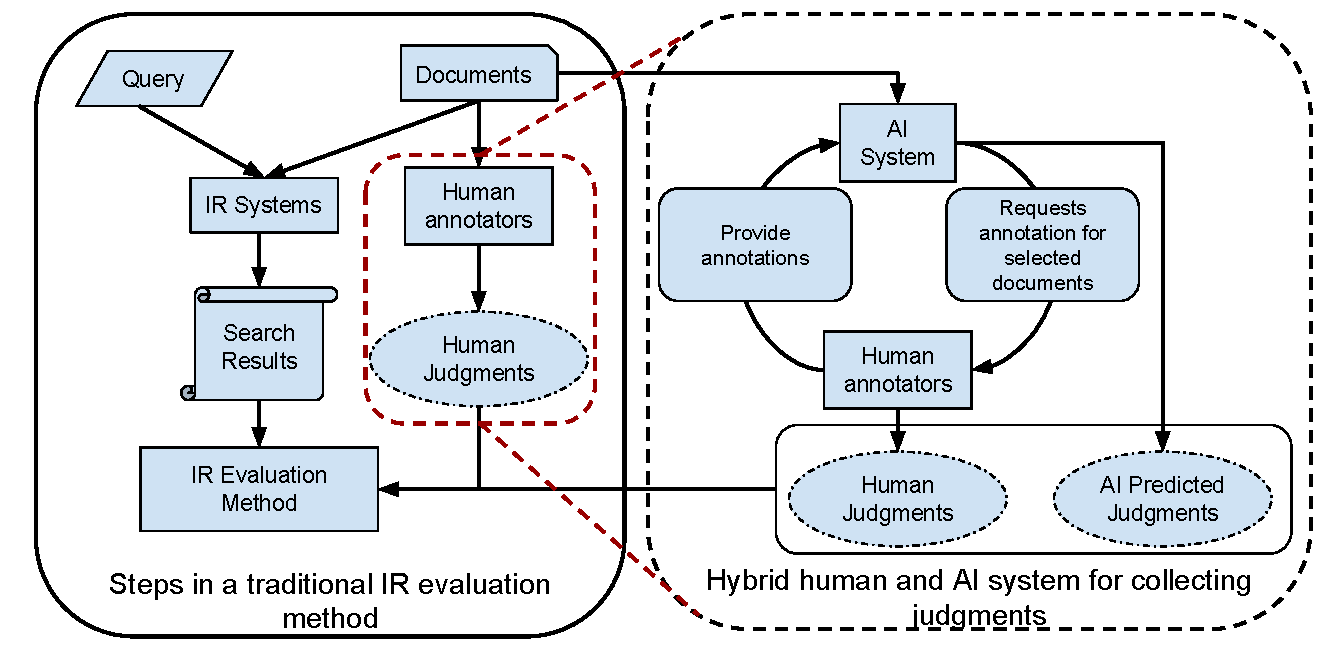
\includegraphics[width=1.0\textwidth]{AI_human_systems.pdf}} 
\vspace{-.5em}
\caption{{\bf Left.} Traditional IR evaluation reliant entirely on manual judging of search results. {\bf Right.} My proposed hybrid human and AI system to collect accurate relevant judgments more efficiently.}
\label{Figure:IR_evaluation}
\end{figure*}





\noindent {\bf Current Work (2 of 2):} 
In the aforementioned JASIS\&T submission, my method focused on intelligent selection of a minimal set of search results for human annotators to judge for search query. In another line of research, I aim at predicting how human judging effort can be intelligently allocated across different search queries. These two lines of work are complementary: both seek to use human effort as judiciously as possible, maximizing the value of the evaluation dataset produced while simultaneously minimizing the human judging cost required to develop it. Whereas traditional approaches allocate the same human judging effort across different search queries, I utilize an AI technique known as {\it reinforcement learning} to predict the number of human relevance judgments which should be collected for each search query. Results show that, my proposed approach can find, on average, $90\%$ of the relevant
search results using 52\% fewer human judgments. This work \cite{Rahman:2019:TestCollection} is currently under review for the World Wide Web (WWW 2019) conference. \\ 



%Existing IR evaluation methods based on a test collection allocate an equal amount of budget for relevance judgment for each of the search topics. However, different search topics have different judgment needs. Thus, allocating a fixed pre-defined budget for all topics may incur more cost than required for topics. Consequently, I realize that developing a low-cost IR test collection requires not only careful selection of documents for human judgment but also intelligent budget allocation across search topics. However, in the absence of a shared task, allocating a budget across topics is again a challenging task as we have no document rankings with which to apply pooling to get an estimated budget for a topic. Since any prior knowledge about the required budget for a topic is not known in advance, in my second research project, I frame this problem as an exploration-exploitation problem with a goal of finding more relevant documents at a lower cost. The exploration-exploitation dilemma arises naturally because for some topics we need more budget than the other topics (i.e. exploitation); however, we also need to make sure that the other topics, that demand less budget, receive a sufficient amount of budget (i.e. exploration). As a result, I adopt a multi-armed bandit method, which is a reinforcement learning technique, to maximize the number of relevant documents under this exploration-exploitation condition. 

\noindent{\bf Additional Work:} While at UT Austin, I have also co-authored several other articles in addition to those described above. One peer-reviewed article \cite{onal2018}, published in the Journal of Information Retrieval, extends an earlier technical report  \cite{DBLP:journals/corr/ZhangRBDCKMABKM16} in providing a literature review of the state-of-the-art in {\it deep learning} AI approaches for IR. Another conference paper \cite{Bhattacharyya:2017:PCW:3022198.3026357}, published at the Association for Computing Machinery (ACM) Computer-Supported Cooperative Work and Social Computing (CSCW) conference, investigates how human judgments of word similarity are impacted by how the textual prompts are presented to the judges. 
Finally, while not performed while at UT Austin, I note that during my Master of Computer Science at the University of Virginia, I also  published a first-authored peer-reviewed article \cite{Rahman:2016:HTS:2872427.2883072} at the 2016 World Wide Web (WWW) conference. This work presents a novel combination of AI modeling techniques (latent Dirichlet allocation and hidden markov models) in order to accurately infer the human sentiment underlying a textual document.\\


\noindent{\bf Future Work:} As stated at the beginning of the proposal, my doctoral research focuses on developing low-cost IR evaluation methods by integrating AI techniques with human annotation. %My ongoing research projects focus on innovating more sophisticated IR evaluation methods. 
One future direction I am interested to pursue investigates how people use different queries to search for the same information. Prior work has shown that
accuracy of IR systems can vary greatly across different queries, yet current evaluation methods typically only consider a single query for each user's search goal. Consequently, I am investing whether we should allocate more human effort during IR system evaluation in developing a broader set of queries on which to evaluate IR systems (i.e. breadth), rather than current practice of judging many documents for fewer queries (i.e. depth). As another direction of future research, {\it crowdsourcing} has recently emerged as an alternative, low-cost way to collect many human judgments at a significantly lower cost than required by traditional human labor models. However, crowdsourced human judgments are also often less reliable than those collected via traditional labor practices. Consequently, I would like to investigate whether we can develop an intelligent AI model which can combine resources from both experts and crowd workers and thus reduce costs even further.  \\


%Since an information need described under a search topic can be expressed using multiple search queries, I am working on finding the best query for a search topic to further reduce the cost. In another research project, I am focusing on reducing the number of judgments needed in a seed set by exploring the possibility of utilizing the description of the topic as an alternative seed document. I am also investigating whether it is possible to utilize a generic cross topic learning model, which is developed using a separate, completely annotated dataset (e.g. LETOR dataset), instead of the existing per topic weak learning model during the early stages of active learning for selecting documents.\\

\noindent{\bf Biographical sketch:} I am a 3rd year PhD student in the School of Information. Prior to coming to UT Austin, I earned my Master of Computer Science from the University of Virginia.
Beyond my research experiences to date at UT Austin, I have sought out and obtained valuable industrial research experiences. During the summer of 2017, at Los Alamos National Laboratory, I developed an AI model to automatically extract clinical information from cancer pathology reports. While at Samsung Research in summer 2018, I worked on improving the question answering module of digital assistants (e.g. Samsung's Bixby, Apple's Siri, etc.)  by integrating an AI-based IR system. These experiences have provided me with additional research training and skill development that will enable me to more successfully execute my planned research. \\

\noindent{\bf Professional Goals:} My long-term career goal is to work as an information retrieval researcher, either as a faculty member at a renowned university or as a research scientist at a respected industry research lab, such as Microsoft Research. \\


\noindent {\bf Financial Need:} My PhD adviser has supported me as a graduate research assistant (GRA) for the past two and a half years. Although he is actively applying for grants to fund me, currently he has no grant funding for the next academic year. As a result, the University Graduate Continuing Fellowship would enable me to continue to focus on advancing my research in the next academic year while my adviser seeks grants to fund me for the subsequent years.      

%\bibliographystyle{unsrtnat}
%\bibliographystyle{ACM-Reference-Format}
\bibliographystyle{IEEEtran}
\bibliographystyle{abbrvnat}
\bibliography{references}


\end{document}
